\documentclass{article}
\usepackage{amssymb}
\usepackage{tikz}
\usepackage[margin=4cm]{geometry}
\setlength{\parskip}{10pt}

\title{Modelos Discretos: Respuestas tarea 1}
\author{Francisco Carvajal, Vicente Díaz, Benjamín Farías}

\begin{document}
\maketitle

\section{Inducción Estructural}
\subsection{Primero definimos la función $Insert(L,k)$}
Usando las definiciones de $Lista$ y $Pre(L)$ vistas en clases, y asumiendo que $L$ está ordenada, definiremos $Insert(L,k)$ como:
\[Insert(\emptyset,k) = \emptyset \rightarrow k\]
\[Insert(L,k)\ = \left\{\begin{array}{lr}
  L \rightarrow k, & k \ge Tail(L)\\
  Insert(Pre(L),k) \rightarrow Tail(L), & k < Tail(L)
\end{array}\right\}
\]

\subsection{Definimos $InsertSort(L)$}

\section{Inducción sobre strings}

\subsection{Definición}
Considere el conjunto \(S\) de secuencias (o strings) compuestas por símbolos 0 y 1, definido por inducción de la siguiente manera:
\begin{itemize}
\item 01 es una secuencia en \(S\).
\item Si u es una secuencia en \(S\), entonces la secuencia 0\(u\)1 está en \(S\).
\item Si \(u\) y \(v\) son secuencias en \(S\), entonces la secuencia \(uv\) está en S.
\end{itemize}

\noindent Por ejemplo, las secuencias 0011 y 0101 están en S.

\subsection{Demostración de la secuencia 00011101}
Se puede demostrar que la secuencia pertenece al conjunto \(S\) usando las reglas dadas, logrando llegar a la conclusión de que es una extensión del caso base.

\noindent Dado que \(uv\) está en \(S\), podemos usar \(u\) como 000111 y \(v\) como 01. \(v\) está en \(S\) porque es el caso base.

\textbf{PDQ:} \(u\) es una secuencia en \(S\).

\noindent Dado que 0\(u\)1 es una secuencia en \(S\), podemos cambiar nuestro \(u\) a 0011. Podemos repetir esto, y ahora \(u\) sería 01, que es el caso base.

\noindent Con esto se demuestra que la secuencia 00011101 se encuentra en el conjunto \(S\).

\subsection{Demostración que todas las secuencias tienen igual cantidad de 0's y 1's}
\(\#0_u\) = Cantidad de 0 en la secuencia \(u\)

\subsubsection*{\emph{B.I.}}
\(u\) = 01

\noindent La secuencia \(u \in S\).

\[\#0_u = 1\ \land\ \#1_u = 1\]

\[\therefore \#0_u = \#1_u\]

\subsubsection*{\emph{H.I.}}
Asumimos que para \(u \in S\ \rightarrow\ \#0_u = \#1_u\).

\textbf{PDQ:} \(\#0_{uv} = \#1_{uv}\ \land\ \#0_{0u1} = \#1_{0u1}\)

\[\#0_{0u1} = \#0_u + 1\ \land\ \#1_{0u1} = \#1_u + 1\]

\[\#0_u = \#1_u\]

\[\therefore \#0_{0u1} = \#1_{0u1}\]

\noindent Ahora falta demostrar que \(\#0_{uv} = \#1_{uv}\):

\[\#0_{uv} = \#0_u + \#0_v\ \land\ \#1_{uv} = \#1_u + \#1_v\]

\[\#0_u = \#1_u\]

\noindent Y como \(v \in S\):

\[\#0_v = \#1_v\]

\[\therefore \#0_{uv} = \#1_{uv}\]

\subsection{Demostración que 11010001 no está en \(S\)}
\subsubsection*{\emph{Propiedad}}
Toda secuencia que pertenezca a \(S\) comienza por el carácter 0.

\subsubsection*{\emph{B.I}}
La secuencia 01 comienza por 0.

\subsubsection*{\emph{H.I}}
Aceptamos la propiedad como verdadera para \(u \in S\).

\textbf{PDQ:} \(0u1\) cumple y que \(uv\) también cumple.

\noindent \(0u1\) comienza por 0 sin importar la secuencia \(u\).

\noindent En \(uv\) la secuencia \(u\) cumple la propiedad, lo que significa que \(uv\) también cumple la propiedad.

\subsubsection*{\emph{Conclusión}}
La secuencia 11010001 no cumple esta propiedad, por tanto no pertenece al conjunto \(S\).

\section{Definición inductiva de grafos}
%Pancho Tarea

\subsection{Mediante inducción estructural defina la estructura del grafo.}
Debemos definir un grafo de a través de la inducción estructural, con base en 
las instrucciones se usará una lista de adyacencia, por lo tanto, lo primero que
debemos crear es una lista de números para que posteriormente el grafo sea una 
lista de listas de números. Se define la lista y algunas funciones útiles.

\subsubsection*{\emph{Lista de naturales}}
\textbf{Definición:}
\[ \emptyset \in \mathcal{L}_{\mathbb{N}} \]
\[ L \in \mathcal{L}_\mathbb{N} \Rightarrow L \rightarrow k \in \mathcal{L}_\mathbb{N}, \forall k \in \mathbb{N}\]
\textbf{Operaciones:}
\[ Insertar(L, k) = L \rightarrow k\]
\newline
\textbf{Ejemplos:}

\[ \rightarrow 0 \rightarrow 2 \rightarrow 7 \]
\[ Insertar(\rightarrow 0 \rightarrow 2 \rightarrow 7, 10) =  \rightarrow 0 \rightarrow 2 \rightarrow 7 \rightarrow 10\]
\[ Insertar(\emptyset, 4) = \rightarrow 4 \]

\subsubsection*{\emph{Definición del grafo}}
Ahora se crea el grafo utilizando la lista, es importante notar que la definición 
de este grafo, es la implementación de un grafo direccional, las listas 
de adyacencia por lo general son para grafos dirigidos. Haremos que sea un grafo
no dirigido posteriormente con el método de $InsertarNodo$, ya que, ese método creara 
una conexión de i a j y de j a i, manteniendo las propiedades de un grafo no dirigido
\footnote{A excepción de que en este grafo la cantidad flechas será el doble que la 
cantidad de aristas reales en el grafo.}. Se utilizará una flecha diferente a la 
de la lista para distinguirlas.

\emph{Definición}

\[ \emptyset \in \mathcal{G} \]
\[ G \in \mathcal{G} \Rightarrow G \rightarrowtail (l) \in \mathcal{G} , \forall l \in \mathcal{L}_\mathbb{N} \]

Ejemplos:

\[ \rightarrowtail ( \rightarrow 2 \rightarrow 3) \rightarrowtail (\rightarrow 3) \rightarrowtail (\rightarrow 0) \rightarrowtail (\rightarrow 0 \rightarrow 1) \]
Representa el siguiente grafo: 

\begin{center}
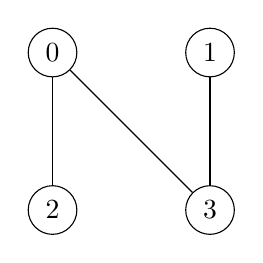
\begin{tikzpicture}
  % Nodos
  \node[circle, draw] (0) at (0,0) {0};
  \node[circle, draw] (1) at (2,0) {1};
  \node[circle, draw] (2) at (0,-2) {2};
  \node[circle, draw] (3) at (2,-2) {3};
  
  % Aristas
  \draw (0) -- (2);
  \draw (0) -- (3);
  \draw (1) -- (3);
\end{tikzpicture}
\end{center}

\subsection{Insertar Nodo}
Esta parte se complica un poco, al ser un grafo no dirigido, ya que, no se puede
solo añadir la lista al final del grafo que ya tenemos, porque se crearía 
asimetría en los datos del grafo, es decir, se puede llegar de j a i, pero 
no de i a j.
Por lo tanto, lo que debemos hacer es añadir la lista al final, pero además 
debemos agregar en cada lista del grafo que corresponda, un borde a la nueva 
arista.
Para hacer esto lo primero que haré es una función que conecte el nodo i y j
de un grafo G.

\[ Conectar((L) \rightarrowtail G, 0, j) = (Insertar(L, j)) \rightarrowtail G \]
\[ Conectar((L) \rightarrowtail G, i, j) = (L) \rightarrowtail Conectar(G, i-1, j) \]

Además, ahora sería útil una función que conecte una lista de nodos a un nodo,
para utilizarla en la función final.

\[ ConectarTodos(G, \emptyset, j) = G  \]
\[ ConectarTodos(G, i \rightarrow L, j) = ConectarTodos(Conectar(G, i, j), L, j)  \]

Ahora que ya podemos conectar el nodo i con el j, necesitamos saber qué valor 
tendrá j, por lo tanto, tenemos que saber cuantos nodos hay en el grafo para 
conocer cuál será el valor del siguiente.

\[ ContarNodos(\emptyset) = 0 \]
\[ ContarNodos((L) \rightarrowtail G) = 1 + ContarNodos(G) \]

Con estas funciones auxiliares creadas, el trabajo se facilita mucho y ya 
podemos definir la función InsertarNodo.

\[ InsertarNodo(G, L) = ConectarTodos(G \rightarrowtail (L), L, ContarNodos(G)) \]

\subsection{Cantidad mínima de aristas}

Debemos demostrar $ a_n = n - 1 $ donde $ a_n $ es la mínima cantidad de aristas
necesarias para conectar n nodos.

\subsubsection*{\emph{B.I.}}
\[ n = 1 \]

\begin{center}
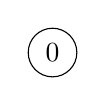
\begin{tikzpicture}
  % Nodos
  \node[circle, draw] (0) at (0,0) {0};
\end{tikzpicture}
\end{center}
En este caso hay 0 aristas, lo que concuerda con $a_1 = 1 - 1 = 0$. :)

\[ n = 2 \]

\begin{center}
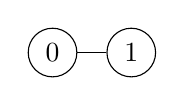
\begin{tikzpicture}
  % Nodos
  \node[circle, draw] (0) {0};
  \node[circle, draw] (1) [right of=0] {1};

  \draw (0) -- (1);
\end{tikzpicture}
\end{center}
En este caso hay 1 arista, lo que concuerda con $a_2 = 2 - 1 = 1$. :)


\[ n = 5 \]

\begin{center}
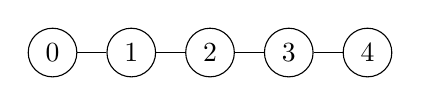
\begin{tikzpicture}
  % Nodos
  \node[circle, draw] (0) {0};
  \node[circle, draw] (1) [right of=0] {1};
  \node[circle, draw] (2) [right of=1] {2};
  \node[circle, draw] (3) [right of=2] {3};
  \node[circle, draw] (4) [right of=3] {4};

  \draw (0) -- (1);
  \draw (2) -- (1);
  \draw (2) -- (3);
  \draw (4) -- (3);
\end{tikzpicture}
\end{center}
En este caso hay 4 aristas, lo que concuerda con $a_5 = 5 - 1 = 4$. :)

\subsubsection*{\emph{H.I.}}
Ahora vamos asumir que $ a_n = n - 1 $.

\subsubsection*{\emph{T.I.}}
PDQ: $a_{n+1} = (n + 1) -1 = n$ \\
Partimos de un grafo que ya estaba mínimamente conectado, y queremos añadir un
nodo. Tenemos que añadirlo con la mínima cantidad de aristas posibles, esto se
hace conectándolo con cualquier nodo que estuviese originalmente en el grafo,
ya que así solo añadimos 1 arista, lo cual es mínimo. Cuando hayamos hecho
esto, el número total de aristas se habrá incrementado en 1 al igual que lo
hará la cantidad nodos, con relación al grafo inicial.

\[\therefore a_{n+1} = a_{n} + 1\]
Por H.I
\[a_{n+1} = (n - 1) + 1\]
\[a_{n+1} = n\]
 

\subsection{Cantidad máxima de aristas}
Debemos demostrar $a_n = \frac{n(n-1)}{2} $ donde $a_n$ es la máxima cantidad de 
aristas que podemos utilizar para conectar n nodos.

\subsubsection*{\emph{B.I}}
\[ n = 1 \]

\begin{center}
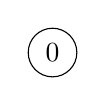
\begin{tikzpicture}
  % Nodos
  \node[circle, draw] (0) at (0,0) {0};
\end{tikzpicture}
\end{center}
En este caso hay 0 aristas, lo que concuerda con $a_1 = \frac{1(1-1)}{2} = 0$. :)

\[ n = 2 \]

\begin{center}
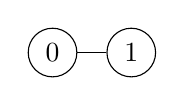
\begin{tikzpicture}
  % Nodos
  \node[circle, draw] (0) {0};
  \node[circle, draw] (1) [right of=0] {1};

  \draw (0) -- (1);
\end{tikzpicture}
\end{center}
En este caso hay 1 arista, lo que concuerda con $a_2 = \frac{2(2-1)}{2} = 1$. :)


\[ n = 5 \]

\begin{center}
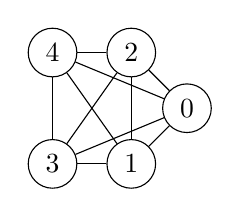
\begin{tikzpicture}
  % Nodos
  \node[circle, draw] (0) {0};
  \node[circle, draw] (1) [below left of=0] {1};
  \node[circle, draw] (2) [above left of=0] {2};
  \node[circle, draw] (3) [left of=1] {3};
  \node[circle, draw] (4) [left of=2] {4};

  \draw (0) -- (1);
  \draw (0) -- (2);
  \draw (0) -- (3);
  \draw (0) -- (4);
  \draw (1) -- (2);
  \draw (1) -- (3);
  \draw (1) -- (4);
  \draw (2) -- (3);
  \draw (2) -- (4);
  \draw (3) -- (4);
\end{tikzpicture}
\end{center}
En este caso hay 10 aristas, lo que concuerda con $a_5 = \frac{5(5-1)}{2}$ = 10. :)

\[ n = 6 \]

\begin{center}
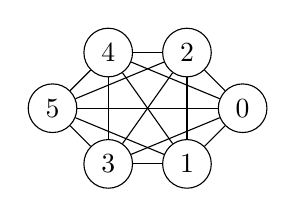
\begin{tikzpicture}
  % Nodos
  \node[circle, draw] (0) {0};
  \node[circle, draw] (1) [below left of=0] {1};
  \node[circle, draw] (2) [above left of=0] {2};
  \node[circle, draw] (3) [left of=1] {3};
  \node[circle, draw] (4) [left of=2] {4};
  \node[circle, draw] (5) [below left of=4] {5};

  \draw (0) -- (1);
  \draw (0) -- (2);
  \draw (0) -- (3);
  \draw (0) -- (4);
  \draw (1) -- (2);
  \draw (1) -- (3);
  \draw (1) -- (4);
  \draw (2) -- (3);
  \draw (2) -- (4);
  \draw (3) -- (4);
  \draw (5) -- (0);
  \draw (5) -- (1);
  \draw (5) -- (2);
  \draw (5) -- (3);
  \draw (5) -- (4);
\end{tikzpicture}
\end{center}
En este caso hay 15 aristas, lo que concuerda con $a_6 = \frac{6(6-1)}{2} = 15$. :)


\subsubsection*{\emph{H.I}}
Ahora asumiremos correcto que:
\[ a_n = \frac{n(n-1)}{2} \]

\subsubsection*{\emph{T.I}}
\emph{PDQ:}
\[ a_{n+1} = \frac{(n+1)((n+1) - 1)}{2} = \frac{(n+1)n}{2} \]
Si tenemos un grafo que está máximamente conectado con n nodos y queremos añadir
uno nuevo, podemos añadir como máximo n aristas, ya que, será añadida una conexión a 
cada nodo que ya estaba en el grafo, no podemos añadir más debido todas las otras 
ya están en el grafo por estar máximamente conectado.
\[ \therefore a_{n+1} = a_n + n \]
\emph{Por H.I.}
\[ a_{n+1} = \frac{(n-1)n}{2} + n = \frac{(n-1)n + 2n}{2} = \frac{n(n-1+2)}{2} = \frac{(n+1)n}{2} \]


\section{Inducción para resolver sumatorias}

\section{Inducción sobre fórmulas lógicas}
\subsection{Tautologías usadas en la demostración}
\begin{enumerate}
  \item Transformación:  $p \rightarrow q \equiv \neg p \lor q$
  \item Distributividad: $p \lor (q \land r) \equiv (p \lor q) \land (p \lor r)$
  \item Distributividad: $p \land (q \lor r) \equiv (p \land q) \lor (p \land r)$
  \item Doble negación: $\neg\neg p \equiv p$
\end{enumerate}

\subsection{Demostración}
Usando inducción demostraremos que si $L(P)$ es un lenguaje proposicional, la fórmula $(\bigvee _{i=1}^{n} X_i) \rightarrow Y $ es lógicamente equivalente a $\bigwedge _{i=1}^{n} (X_i \rightarrow Y)$,
para todo $n \ge 1$.
\subsubsection*{\emph{B.I}}
\emph{n=1}
\[X_1 \rightarrow Y \equiv X_1 \rightarrow Y\]
\emph{n=2}
\[(X_1 \lor X_2) \rightarrow Y \qquad (X_1 \rightarrow Y) \land (X_2 \rightarrow Y) \]
\[\neg(X_1 \lor X_2) \lor Y \qquad (\neg X_1 \lor Y) \land (\neg X_2 \lor Y) \]
\[(\neg X_1 \land \neg X_2) \lor Y \quad \equiv \quad (\neg X_1 \land \neg X_2) \lor Y \]

\subsubsection*{\emph{H.I}}
\[ (\bigvee _{i=1}^{n} X_i) \rightarrow Y \equiv \bigwedge _{i=1}^{n} (X_i \rightarrow Y) \]

\subsubsection*{\emph{T.I}}
Para demostrar que lo propuesto en el enunciado se cumple, podemos usar el $PIS$ en lo siguiente:\\
\emph{Empezaremos por la fórmula lógica de la derecha}
\[ (\bigvee _{i=1}^{n+1} X_i) \rightarrow Y \equiv \bigwedge _{i=1}^{n+1} (X_i \rightarrow Y) \]

\emph{Aplicamos propiedad de la "ANDatoria"}
\[ \bigwedge _{i=1}^{n+1} (X_i \rightarrow Y) = \bigwedge _{i=1}^{n} (X_i \rightarrow Y) \land (X_{n+1} \rightarrow Y) \]

\emph{Por H.I}
\[ \bigwedge _{i=1}^{n} (X_i \rightarrow Y) \land (X_{n+1} \rightarrow Y) = ((\bigvee _{i=1}^{n} X_i) \rightarrow Y) \land (X_{n+1} \rightarrow Y) \] 

\emph{Aplicamos Transformación}
\[ ((\bigvee _{i=1}^{n} X_i) \rightarrow Y) \land (X_{n+1} \rightarrow Y) = (\neg(\bigvee _{i=1}^{n} X_i) \lor Y) \land (\neg X_{n+1} \lor Y) \]

\emph{Aplicamos Distributividad}
\[ (\neg(\bigvee _{i=1}^{n} X_i) \lor Y) \land (\neg X_{n+1} \lor Y) = (\neg(\bigvee _{i=1}^{n} X_i) \land \neg X_{n+1} ) \lor Y\]

\emph{Aplicamos Doble negación}
\[ (\neg(\bigvee _{i=1}^{n} X_i) \land \neg X_{n+1} ) \lor Y = \neg\neg(\neg(\bigvee _{i=1}^{n} X_i) \land \neg X_{n+1} ) \lor Y\] 
\[ \neg\neg(\neg(\bigvee _{i=1}^{n} X_i) \land \neg X_{n+1} ) \lor Y = \neg((\bigvee _{i=1}^{n} X_i) \lor  X_{n+1} )\lor Y \]

\emph{Aplicamos propiedad de la "ORatoria"}
\[ \neg((\bigvee _{i=1}^{n} X_i) \lor  X_{n+1}) \lor Y = \neg(\bigvee _{i=1}^{n+1} X_i) \lor Y \]

\emph{Aplicamos Transformación}
\[ \neg(\bigvee _{i=1}^{n+1} X_i) \lor Y = (\bigvee _{i=1}^{n+1} X_i) \rightarrow Y\]

\emph{Ahora es claro que:}
\[ (\bigvee _{i=1}^{n+1} X_i) \rightarrow Y \equiv \bigwedge _{i=1}^{n+1} (X_i \rightarrow Y) \]

\newpage
\section{Inducción sobre números naturales}
Demostraremos lo siguiente:
\[ n_1 + n_2 + ... + n_k = n \]
\[ n_1^2 + n_2^2 + ... + n_k^2 \leq (n-k+1)^2 + k -1\]
La demostración se hará con una inducción sobre k, es decir, el número de 
elementos dentro de la suma.

\subsubsection*{\emph{B.I.}}
$k=0$
\[0 \leq (0 - 0 +1)^2 + 0 -1 = 0\]
$k=1$
\[ n_1^2 \leq (n_1^2 - 1 + 1)^2 + 1 - 1 = n_1^2\]
$k=2$
\[ n_1^2 + n_2^2 \leq (n_1 + n_2 - 2 + 1)^2 + 2 -1 = n_1^2 + 2n_1n_2+n_2^2-2n_1-2n_2+2 \]
\hspace*{0pt}\hfill $/ - n_1^2 - n_2^2$
\[ 0 \leq  2n_1n_2-2n_1-2n_2+2 \]
\[ 0 \leq 2(n_1 - 1)(n_2 - 1) \]
\[ 0 \leq (n_1 - 1)(n_2 -1) \]

\[ 1 \leq n_1 = 0 \leq n_1 - 1  \]
\[ 1 \leq n_2 = 0 \leq n_2 -1  \]
\[ \therefore  0 \leq (n_1 - 1)(n_2 -1)\]

$k=3$
%TODO: Implementar
\subsubsection*{\emph{H.I.}}
Ahora asumiremos lo siguiente como correcto.
\[ n_1^2 + n_2^2 + ... + n_k^2 \leq (n-k+1)^2 + k -1\]


\subsubsection*{\emph{T.I.}}
PDQ:
\[ n_1^2 + n_2^2 + ... + n_k^2 + n_{k+1}^2 \leq ((n + n_{k+1}) - (k+1) + 1)^2 + (k+1)-1 \]
\[ n_1^2 + n_2^2 + ... + n_k^2 + n_{k+1}^2 \leq ((n + n_{k+1}) - k)^2 + k \]
-\[   n_1^2 + n_2^2 + ... + n_k^2 \leq (n-k+1)^2 + k -1\]
=\[ n_{k+1}^2 \leq (n+n_{k+1} - k)^2 + k - ((n-k+1)^2 + k -1) \]
\[ n_{k+1}^2 \leq (n+n_{k+1})^2 - 2k(n+n_{k+1}) + k^2 + k - ((n-k)^2 + 2(n-k) + 1+ k -1) \]
\[ n_{k+1}^2 \leq (n+n_{k+1})^2 - 2k(n+n_{k+1}) + k^2 - ((n-k)^2 + 2(n-k)) \]
\[ n_{k+1}^2 \leq n^2 + 2nn_{k+1} + n_{k+1}^2 - 2kn -2kn_{k+1} + k^2  - (n^2 - 2kn +k^2 + 2n - 2k)) \]
\[ n_{k+1}^2 \leq 2nn_{k+1} + n_{k+1}^2 -2kn_{k+1} - ( 2n - 2k)) \]
\hspace*{0pt}\hfill $/ -n_{k+1}^2 $
\[ 0 \leq 2nn_{k+1} -2kn_{k+1} - 2n + 2k \]
\hspace*{0pt}\hfill $/ \times\frac{1}{2} $
\[ 0 \leq nn_{k+1} -kn_{k+1} - n + k \]
\[ 0 \leq n_{k+1}(n-k) - n + k \]
\[ 0 \leq n_{k+1}(n-k) - (n - k) \]
\[ 0 \leq n_{k+1}(n-k) - (n - k) \]
\[ 0 \leq (n-k)( n_{k+1}-1) \]


\section{Falacias inductivas}
\subsection{Teorema y demostración}
Considere este teorema y su “demostración” por inducción:

\noindent \textbf{Teorema} Dado un conjunto de \(n\) niñas, si al menos una de ellas tiene ojos azules, entonces las \(n\) niñas tienen ojos azules.

\noindent \textbf{Demostración.} Para n = 1 el enunciado es obviamente cierto. Supongamos que la proposición es cierta para n niñas.
Sean \(N_1, ... , N_{n+1}\) niñas con al menos una, pongamos \(N_1\), con ojos azules. Veamos que todas tienen los ojos azules:

\noindent El grupo de niñas \(N_1, ... , N_n\) verifica entonces la hipótesis de inducción, con lo que todas ellas son de ojos azules. Por tanto, como \(N_2\) tiene los ojos azules, tambien \(N_2, ... , N_{n+1}\) verifica la hipótesis de inducción, con lo que dichas niñas y en particular \(N_{n+1}\) tiene los ojos azules. Así pues, \(N_1, ... , N_n, N_{n+1}\) tienen los ojos azules.

\subsection{Error de la demostración}
El error de esta demostración recae en tomar cualquier conjunto con \(n\) niñas y pensar que es igual que otro conjunto con \(n\) niñas. La verdad es que cada conjunto de \(n\) niñas es distinto, ya que pueden tener distintas niñas con distintas características físicas.

\noindent La demostración se cae de inmediato cuando conformo un conjunto con \(n\) niñas que tengan los ojos de color verde, y ahora saco un niña de este conjunto y hago que sea la niña \(N_{n+1}\) del conjunto con niñas de ojos azules. Según el teorema las \(n + 1\) niñas tienen los ojos azules, pero en realidad hay una que tiene los ojos verdes.

\noindent Por esto no se puede asumir que el conjunto conformado por las niñas \(N_1, ... , N_n\) es el mismo que el conjunto con las niñas \(N_2, ... , N_{n+1}\).

\end{document}
